\documentclass[11pt]{article}

\usepackage[margin=1in]{geometry}
\usepackage{graphicx}
\usepackage{booktabs}
\usepackage{amsmath}
\usepackage{amssymb}
\usepackage{siunitx}
\usepackage{microtype}
\usepackage[numbers,sort&compress]{natbib}
\usepackage{hyperref}
\usepackage{xcolor}
\hypersetup{colorlinks=true, linkcolor=blue!40!black, citecolor=blue!50!black, urlcolor=blue!50!black}

\title{Clustered synapses develop in distinct dendritic domains in visual cortex before eye opening}
\author{}
\date{}

\begin{document}
\maketitle

\begin{abstract}
\noindent Synaptic inputs to adult cortical pyramidal neurons are clustered along dendrites so that neighboring synapses carry related information, a geometric arrangement that supports local dendritic nonlinearities and high-fidelity computation. When and how this clustered architecture is assembled during development remains unresolved, particularly at the resolution of individual functional synapses in vivo. To address this gap, we combined whole-cell voltage-clamp recordings with two-photon calcium imaging of GCaMP6s-expressing dendrites in layer 2/3 pyramidal neurons of the mouse primary visual cortex during the second postnatal week, spanning postnatal day (P) 8 to P13 -- the week leading up to eye opening. Across 11 mice and 12 dendritic areas we resolved 354 functional synapses producing 3440 transmission events, and we mapped how functional inputs are spatially and temporally organized along developing dendrites. Synapse density and the frequency of transmission per synapse rose several-fold across the second postnatal week, with spine synapses consistently more active than shaft synapses at both ages ($0.55 \pm 0.09$ vs.\ $0.16 \pm 0.03$ min$^{-1}$ at P8--10; $0.67 \pm 0.07$ vs.\ $0.23 \pm 0.03$ min$^{-1}$ at P12--13). High-activity synapses organized into discrete dendritic domains whose extent, membership, density and coverage roughly doubled during the week (coverage rose from $27.2 \pm 16.2\%$ to $61.3 \pm 29.4\%$), and local co-activity was consistently higher inside than outside these domains (e.g.\ $0.08 \pm 0.02$ vs.\ $0.02 \pm 0.01$ at P8--10). Finally, Mann--Kendall plasticity scores at individual synapses were correlated with their local co-activity, linking synchronization with neighbors to synapse stabilization. Thus functional dendritic domains are assembled before eye opening, providing ready-made computational subunits that could support selective visual processing from the moment the eyes open.
\end{abstract}

\section{Introduction}

Assembling a functional cerebral cortex requires neurons to establish specific synaptic partnerships and then refine them through activity-dependent plasticity \citep{sanes2020synaptic}. In adult sensory cortex, this refinement culminates in a remarkable geometric organization: along short stretches of a pyramidal cell dendrite, neighboring synapses preferentially carry related information. Two-photon mapping of dendritic spines in mouse primary visual cortex (V1) shows that inputs representing nearby locations in visual space are more likely to synapse on neighboring spines \citep{iacaruso2017synaptic}, and in ferret V1, synapses are clustered by orientation preference with the degree of clustering predicting each cell's subthreshold nonlinearity \citep{wilson2016orientation}. Local synchronization between adjacent spines is also evident during spontaneous activity in reduced preparations \citep{takahashi2012locally}. Prior in vivo mapping of dendritic calcium signals has shown that even adult neurons exhibit fine-scale functional structure along their branches \citep{jia2010dendritic}.

This clustering is functionally consequential because pyramidal dendrites integrate nearby coincident inputs supralinearly. Radial oblique dendrites of CA1 pyramidal cells generate NMDA-receptor-dependent dendritic spikes when synchronous inputs converge within tight spatial and temporal windows \citep{losonczy2006integrative}, and analogous regenerative events in vivo amplify stimulus responses and sharpen feature tuning in V1 and barrel cortex \citep{smith2013dendritic,lavzin2012nonlinear}. Spines themselves contribute high-impedance compartmentalization that amplifies unitary inputs and promotes cooperativity between co-active neighbors \citep{harnett2012synaptic}. In this framework the pyramidal neuron behaves as a two-layer network in which each branch computes a local nonlinear subunit \citep{poirazi2003pyramidal,makara2013variable}, and this dendritic associative mechanism is posited to be a general organizing principle of the neocortex \citep{larkum2013cellular}. Manipulations that silence dendritic nonlinearities degrade tuning selectivity, directly coupling subcellular synaptic geometry to perceptual computation \citep{smith2013dendritic,lavzin2012nonlinear,wilson2018differential}.

Despite a strong case for clustering in the mature cortex, developmental studies have left three basic questions unanswered at the resolution of individual functional synapses in vivo. First, when in postnatal development do synaptic inputs become clustered? Second, are synapses deposited already clustered, or are initially random synapses sorted into clusters later? And third, do inputs distribute smoothly along dendrites or concentrate in spatially discrete domains separated by largely inactive stretches? These questions are especially pressing for the second postnatal week in rodents, when synapse density rises steeply and approaches adult levels by the time the eyes open at around postnatal day (P) 14. During this interval the cortex is driven primarily by spontaneous activity -- retinal waves transmitted through the thalamus \citep{ackman2012retinal} together with locally generated cortical patterns \citep{siegel2012peripheral}. Reviews have long proposed that clustering could arise through local activity-dependent plasticity \citep{winnubst2012synaptic}, yet a longitudinal in vivo measurement at single-synapse resolution has been lacking.

We addressed this gap by combining in vivo whole-cell voltage-clamp with two-photon imaging of dendritic calcium transients reported by GCaMP6s \citep{chen2013ultrasensitive} in layer 2/3 pyramidal neurons of the mouse primary visual cortex across P8 to P13. Resonant scanning combined with piezo-driven z-positioning allowed us to sample a much larger fraction of each neuron's dendritic tree than was accessible in prior work, yielding 354 functional synapses and 3440 individual transmission events across 12 dendritic areas from 11 mice. QX-314 in the pipette \citep{takahashi2012locally} and holding the membrane near NMDA-facilitating potentials \citep{jia2010dendritic,svoboda1999spread} enabled detection of transmission at both spine and shaft synapses. Our measurements reveal that functional inputs become organized into spatially and functionally distinct dendritic domains already during the second postnatal week, and that the local co-activity of neighbors correlates with synapse stabilization. Thus clustered inputs are built, not inherited, and the scaffolding is laid down before the first visual experience.

\section{Methods}

\subsection{Animals and in utero electroporation}
All experimental procedures were approved by the Institutional Animal Care and Use Committee of the Royal Netherlands Academy of Arts and Sciences. Eleven C57BL/6J mouse pups between P8 and P13 were used. Constructs were delivered by in utero electroporation at embryonic day 16.5. Pyramidal neurons in layer 2/3 of the visual cortex were co-transfected with GCaMP6s (Addgene plasmid 40753; 2 mg/ml) in pCAGGS and DsRed-Express in pCAGGS (0.5--2 mg/ml) \citep{chen2013ultrasensitive}. Pregnant dams were anesthetized with isoflurane and received a 1.5--2 cm incision in the abdominal wall, after which DNA (1 $\mu$l) was injected into the lateral ventricle of each embryo through a sharp glass pipette. Five square-wave voltage pulses (30 V, 50 ms duration, 950 ms interval) were delivered across the head through tweezer electrodes with conductive gel using a custom electroporator. The uterine horns were rinsed with warm saline, returned to the abdomen, and the muscle and skin layers sutured.

\subsection{In vivo electrophysiology and two-photon imaging}
Surgical preparation and head fixation for in vivo imaging followed our published protocols \citep{siegel2012peripheral}. Animals were induced with 2\% isoflurane, reduced to 0.7--1\% during recording. BSA--Alexa 594-coated glass electrodes (4.5--6 M$\Omega$) were advanced into layer 2/3 for targeted whole-cell recordings. The intracellular solution contained 120 mM CsMeSO$_3$, 8 mM NaCl, 15 mM CsCl$_2$, 10 mM TEA-Cl, 10 mM HEPES, 5 mM QX-314 bromide, 4 mM MgATP, and 0.3 mM Na-GTP, which suppressed somatic action potentials while preserving synaptic currents \citep{takahashi2012locally}. Currents were recorded at 10 kHz and low-pass filtered at 3 kHz with a Multiclamp 700B (Molecular Devices). Neurons were held at $-30$ mV to facilitate NMDA-receptor-mediated calcium influx at individual synapses \citep{jia2010dendritic,svoboda1999spread}. Two-photon imaging was performed on a Nikon A1R-MP microscope equipped with a 16$\times$/0.8-NA water-immersion objective and a Chameleon II Ti:sapphire laser (Coherent). Dendrites were imaged at 5--15 Hz with a pixel size of $0.32$ $\mu$m in single planes or thin stacks (plane spacing 1.5--2 $\mu$m). The schematic in Figure~\ref{fig:setup} illustrates this configuration. Barrages of somatic current were identified as fast-rising inward events of at least 10 pA that consisted of multiple synaptic currents and were separated by at least 3 s.

\subsection{Image processing and synapse identification}
Recordings were drift-corrected using NoRMCorre \citep{pnevmatikakis2017normcorre}, and $\Delta F$ stacks were computed using the mean pixel fluorescence as baseline. Regions of interest corresponding to putative synapses were drawn by hand in ImageJ at sites where spines were visible or where local calcium transients were observed, with additional ROIs placed across intervening dendritic segments to minimize missed events. Candidate synaptic transmission events were initially flagged as mean fluorescence increases exceeding twice the local noise level, then confirmed by manual review requiring a stable local fluorescence maximum lasting at least two frames and no coincidence with movement. Events in lateral spine appendages were labeled spine events, while events in smooth shaft stretches were labeled shaft events; ambiguous cases were resolved using 3D reconstructions from z-stacks. Only synaptic sites active at a transmission frequency of at least 0.03 min$^{-1}$ were retained.

\subsection{Structural, domain, and statistical analyses}
To test whether synapse positions were structured or random along the dendrite, we first assigned ``empty'' positions between measured synapses such that the entire imaged dendrite was tiled with real or empty positions at the typical minimal inter-synapse spacing ($4 \pm 1$ $\mu$m). Distances between all real and empty locations were computed using Matlab's shortest-path-with-obstacle-avoidance routine, real synapses were shuffled across real and empty positions, and the distances from each synapse to its nearest proximal and distal neighbors were compared between observed and 100 shuffled distributions using a Kolmogorov--Smirnov test. Co-activity of a synapse with a reference group (e.g.\ neighbors within 10 $\mu$m, within the same domain, or in other domains) was computed as the number of transmission events of the reference group that occurred in the same barrages as the synapse's events, divided by the synapse's total events and normalized by the size of the reference group. This definition follows directly from prior work showing that co-transmission during barrages is the key substrate of local plasticity in developing cortex \citep{winnubst2012synaptic}.

High-activity synapses were defined for each age group as those in the top 20\% of transmission frequency. A dendritic domain contained at least one high-activity synapse; additional high-activity synapses within 10 $\mu$m were assigned to the same domain, and normal synapses within 10 $\mu$m of a high-activity synapse were included as domain members. Normal synapses lying between two high-activity synapses from distinct domains and within 20 $\mu$m of the split were assigned to the closer domain. Domain extent was measured as the distance between a domain's most distal members and padded by 5 $\mu$m at each edge when no normal members extended beyond the bounding high-activity synapse; thus a minimal single-synapse domain had an extent of 10 $\mu$m. We used 2-sided paired and independent Student's $t$-tests for normally distributed data and for low-$n$ samples where normality tests are underpowered, Mann--Whitney $U$ tests for independent non-normal samples, Wilcoxon signed-rank tests for paired non-normal samples, linear regression to test age dependence, and Kolmogorov--Smirnov tests to compare distributions. Temporal trends in per-synapse transmission frequency were summarized with the Mann--Kendall trend statistic.

\section{Results}

\subsection{Mapping functional synaptic inputs onto spine and shaft synapses}

To capture functional synaptic inputs at individual-synapse resolution in vivo, we co-expressed GCaMP6s and DsRed in layer 2/3 pyramidal neurons of the mouse primary visual cortex and recorded from them in whole-cell voltage-clamp mode while imaging their dendritic calcium transients with two-photon microscopy (Figure~\ref{fig:setup}). Resonant scanning combined with piezo-driven z-positioning allowed us to sample a large proportion of the dendritic tree from each neuron. Across 11 mice imaged between P8 and P13, we mapped 354 functional synapses on 12 dendritic areas and recorded 3440 individual synaptic transmission events. Simultaneous voltage-clamp recordings provided a parallel readout of the barrages of synaptic currents impinging on the soma while the imaged dendrites reported transmission at specific synapses.

Because many cortical synapses during this developmental window are located directly on the dendritic shaft rather than on spines \citep{winnubst2012synaptic}, we suppressed somatic action potentials with QX-314 in the pipette and held neurons at $-30$ mV to facilitate NMDA-receptor activation \citep{takahashi2012locally,jia2010dendritic,svoboda1999spread}. Under these conditions we could resolve local calcium transients at both spine and shaft synapses without interference from back-propagating action potentials. This configuration allowed us to distinguish spine events, which appeared as focal transients in small lateral appendages of the dendrite, from shaft events, which appeared as localized transients in smooth dendritic stretches; ambiguous cases were disambiguated from 3D image stacks. Together, this approach provided the longitudinal, high-resolution view of synaptic inputs required to ask how clustering emerges in the developing cortex.

\subsection{Synaptic inputs increase rapidly during the second postnatal week}

Having validated our ability to resolve transmission at individual spine and shaft synapses, we first asked how the complement of functional synaptic inputs changes across the second postnatal week. Using linear regression across $n = 12$ experiments, we found that the density of functional synapses along imaged dendrites increased significantly with age, as did the mean transmission frequency per synapse. Correspondingly, the total number of synaptic transmission events sampled per dendrite was higher by P12--13 ($n = 6$ dendrites) than at the beginning of the second postnatal week (P8--10, $n = 6$ dendrites). Despite this functional growth, the fraction of synapses located on spines did not change significantly across the sampled ages, consistent with prior evidence that spine densities continue to rise beyond P14 in mouse V1.

\begin{figure}[htbp]
\centering
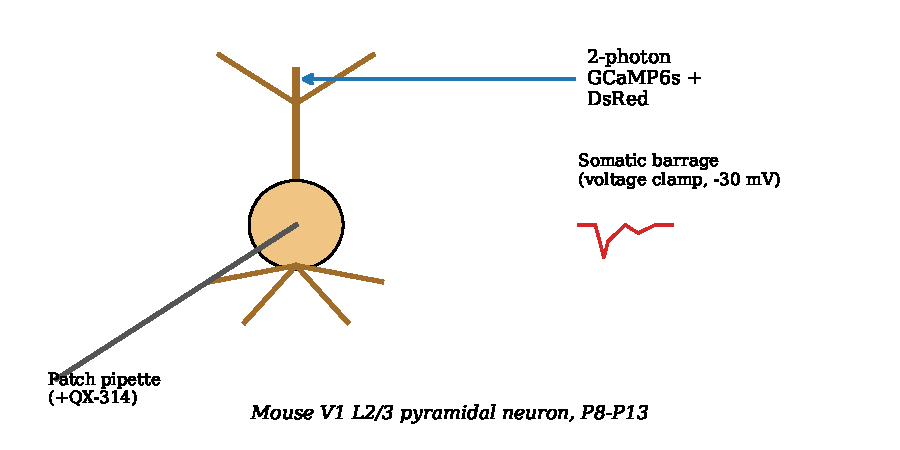
\includegraphics[width=0.75\textwidth]{figures/fig_setup_schematic.pdf}
\caption{Experimental configuration. Layer 2/3 pyramidal neurons in mouse primary visual cortex were targeted in vivo for whole-cell voltage-clamp recording under two-photon guidance. GCaMP6s and DsRed were delivered by in utero electroporation at embryonic day 16.5, and QX-314 in the internal solution blocked somatic action potentials. Holding the neuron at $-30$ mV facilitated NMDA-receptor-dependent calcium transients at both spine and shaft synapses.}
\label{fig:setup}
\end{figure}

Synapse-level transmission rates were strikingly heterogeneous. The distribution of per-synapse transmission frequencies was very long-tailed: most synapses fired only rarely, but a small fraction were highly active. Within this distribution, spine synapses were systematically more active than shaft synapses at both ages ($0.55 \pm 0.09$ min$^{-1}$ at spines vs.\ $0.16 \pm 0.03$ min$^{-1}$ at shafts in P8--10; $0.67 \pm 0.07$ min$^{-1}$ vs.\ $0.23 \pm 0.03$ min$^{-1}$ at P12--13; mean $\pm$ SEM; Mann--Whitney $U$ test, $p < 10^{-9}$ at both ages; P8--10: $n = 36$ spine vs.\ $113$ shaft synapses; P12--13: $n = 83$ spine vs.\ $122$ shaft synapses; Figure~\ref{fig:rates}). At the same time, a fraction of structurally identifiable spines did not transmit during our recordings -- $25 \pm 20\%$ in younger and $9 \pm 9\%$ in older dendrites (mean $\pm$ STD; mean recording durations $29 \pm 8$ and $26 \pm 6$ min, respectively) -- consistent with a population of presynaptically silent synapses at these ages. Taken together, these observations show that synapse density, per-synapse activity, and the asymmetry between spine and shaft rates all grow rapidly across the second postnatal week, setting the stage for the emergence of larger-scale organization.

\begin{figure}[htbp]
\centering
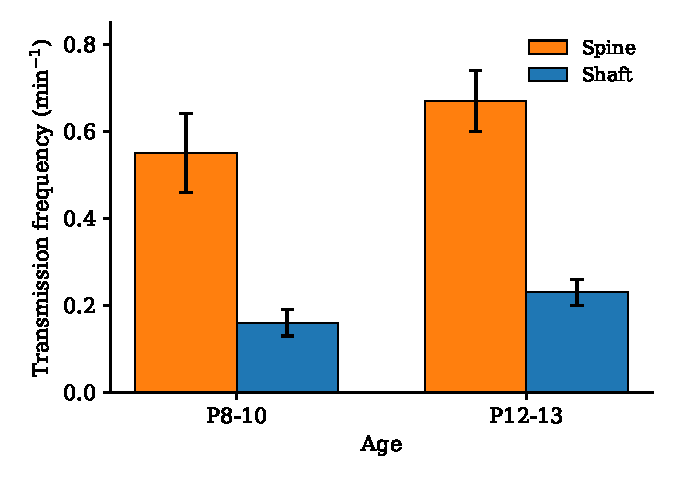
\includegraphics[width=0.55\textwidth]{figures/fig_transmission_rates.pdf}
\caption{Spine synapses sustained higher transmission rates than shaft synapses at both developmental stages (P8--10: spine $0.55 \pm 0.09$ min$^{-1}$ vs.\ shaft $0.16 \pm 0.03$ min$^{-1}$; P12--13: spine $0.67 \pm 0.07$ min$^{-1}$ vs.\ shaft $0.23 \pm 0.03$ min$^{-1}$; mean $\pm$ SEM; each $p < 10^{-9}$, Mann--Whitney $U$ test; P8--10 $n = 36$ spine and $113$ shaft, P12--13 $n = 83$ spine and $122$ shaft synapses).}
\label{fig:rates}
\end{figure}

\subsection{Synaptic transmission aligns with somatic barrages}

Having established that per-synapse rates rise sharply and remain systematically higher at spines than at shafts, we next asked how the timing of transmission at individual synapses related to the coordinated network events that dominate cortical activity in this developmental window. Simultaneous somatic recordings identified barrages of synaptic currents as transient inward currents of at least 10 pA composed of multiple unitary events. Most synaptic transmission events at the dendrite occurred during these barrages: 59\% in young neurons and 61\% in older neurons. The rate of barrages did not change significantly with age, indicating that overall network activity was comparable at P8--10 and P12--13, but the content of each barrage changed.

Quantitatively, we observed a trend toward higher total synaptic charge transferred per barrage with age, and a significant increase in the number of synaptic transmission events observed per barrage. The number of transmission events per barrage correlated linearly with the charge transferred during that barrage, as expected if each event contributes approximately additively to the somatic integral. More surprisingly, the amplitude of individual synaptic transmission events at a given synapse correlated with barrage size, suggesting that more than one vesicle may be released per synapse during larger coincident network events. These findings indicate that developing synapses do not merely become more numerous and individually active; they also become more coordinated with the larger network, so that downstream integration in the soma reflects increasingly rich coincident input.

\subsection{Synapses are spatially organized along developing dendrites}

These timing measurements established that developing synapses receive and transmit within a coordinated network context. Building on this observation, and on the long-tailed per-synapse rate distribution, the next question was whether the spatial placement of synapses along the dendrite reflected any structure beyond chance. The observation that per-synapse activity was highly non-uniform motivated us to ask whether synapse positions themselves were spatially structured. In young dendrites, we noticed that certain stretches carried multiple active synapses while neighboring stretches were essentially silent. To formalize this impression, we compared the distribution of distances between each synapse and its nearest proximal and distal neighbors with distributions generated by randomly shuffling synapse positions over the available dendritic length. At P8--P10 the observed inter-synapse distance distribution differed significantly from the shuffled distributions (Kolmogorov--Smirnov test), indicating that synapses preferentially accumulated in subsegments of the dendrite. By P12--P13 the observed distribution was indistinguishable from the shuffled distributions, consistent with more uniform coverage of the dendrite once synapse density had risen.

Within this spatial organization, highly active synapses were not randomly placed. We defined high-activity synapses as those in the top 20\% of transmission frequency within each age group. High-activity synapses were predominantly on spines ($76\%$), consistent with the overall higher transmission rates of spine synapses. Critically, they tended to cluster near one another along the dendrite. Synapses located within 10 $\mu$m of a high-activity synapse had a higher mean transmission frequency than synapses farther away ($n = 181$ for within-10-$\mu$m and $n = 173$ for beyond-10-$\mu$m synapses; independent Student's $t$-test), and the activity difference was reproducible across ages. Together these analyses show that functional synapses are already spatially structured in young dendrites, with high-activity synapses serving as anchors around which other active synapses cluster.

\subsection{Synaptic inputs are organized in functional domains}

To formalize the observation that high-activity synapses were surrounded by other active synapses, we defined dendritic domains as contiguous stretches containing at least one high-activity synapse and its active neighbors within 10 $\mu$m. Multiple high-activity synapses within 10 $\mu$m of one another were grouped into a single domain; normal synapses between distant high-activity synapses were assigned to the nearer one. We then asked how these domains evolved across the second postnatal week and whether their members showed the coordinated activity expected of a functional unit (Figure~\ref{fig:domains}).

\begin{figure}[htbp]
\centering
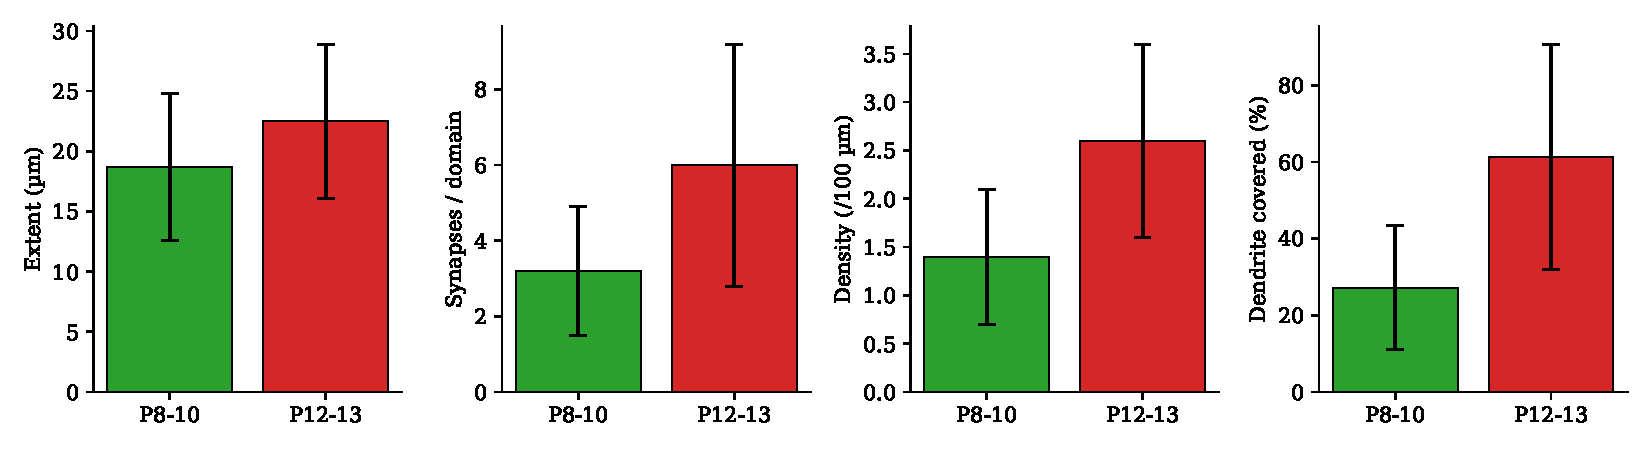
\includegraphics[width=0.95\textwidth]{figures/fig_domain_features.pdf}
\caption{Dendritic domains grew on four axes during the second postnatal week. Extent increased modestly (P8--10: $18.7 \pm 6.1$ $\mu$m; P12--13: $22.5 \pm 6.4$ $\mu$m), while synapses per domain (P8--10: $3.2 \pm 1.7$; P12--13: $6.0 \pm 3.2$) and domain density (P8--10: $1.4 \pm 0.7$; P12--13: $2.6 \pm 1.0$ per 100 $\mu$m) approximately doubled. The fraction of dendritic length covered by domains rose from $27.2 \pm 16.2\%$ to $61.3 \pm 29.4\%$ (mean $\pm$ STD).}
\label{fig:domains}
\end{figure}

Domains grew substantially across the second postnatal week. Their extent increased only modestly (P8--10: $18.7 \pm 6.1$ $\mu$m vs.\ P12--13: $22.5 \pm 6.4$ $\mu$m), but the number of synapses per domain approximately doubled ($3.2 \pm 1.7$ vs.\ $6.0 \pm 3.2$), as did the density of domains along the dendrite ($1.4 \pm 0.7$ per 100 $\mu$m vs.\ $2.6 \pm 1.0$ per 100 $\mu$m). As a consequence, the fraction of dendritic length covered by domains more than doubled ($27.2 \pm 16.2\%$ at P8--10 vs.\ $61.3 \pm 29.4\%$ at P12--13; mean $\pm$ STD). The fraction of all functional synapses that belonged to a domain also rose significantly from $46.2 \pm 7.4\%$ to $72 \pm 23.2\%$ ($n = 6$ dendrites in each age group; $p = 0.026$, $t$-test), so that by the end of the second postnatal week most inputs had been incorporated into a domain. These metrics are summarized in Table~\ref{tab:domains}.

\begin{table}[htbp]
\centering
\caption{Domain features across the second postnatal week. Values are mean $\pm$ STD unless otherwise noted.}
\label{tab:domains}
\begin{tabular}{lcc}
\toprule
Feature & P8--10 & P12--13 \\
\midrule
Extent ($\mu$m) & $18.7 \pm 6.1$ & $22.5 \pm 6.4$ \\
Synapses per domain & $3.2 \pm 1.7$ & $6.0 \pm 3.2$ \\
Density (per 100 $\mu$m) & $1.4 \pm 0.7$ & $2.6 \pm 1.0$ \\
Dendritic length covered (\%) & $27.2 \pm 16.2$ & $61.3 \pm 29.4$ \\
Synapses in domains (\%; $n = 6$) & $46.2 \pm 7.4$ & $72 \pm 23.2$ \\
\bottomrule
\end{tabular}
\end{table}

Domains were not merely spatial constructs but also functional units. The local co-activity of synapses inside domains was consistently higher than that of synapses outside domains at both ages (P8--10: in-domain $0.08 \pm 0.02$, out-of-domain $0.02 \pm 0.01$; P12--13: in-domain $0.06 \pm 0.01$, out-of-domain $0.04 \pm 0.01$; mean $\pm$ SEM; $n = 213$ in-domain, $n = 173$ out-of-domain synapses; Mann--Whitney $U$ test; Figure~\ref{fig:coactivity} and Table~\ref{tab:coactivity}). Moreover, domains were functionally distinct from one another: within-domain co-activity exceeded between-domain co-activity on every imaged dendrite (Wilcoxon signed-rank test), indicating that each domain received a largely private input pattern. These findings demonstrate that the clustered inputs reported in the adult cortex \citep{iacaruso2017synaptic,wilson2016orientation,takahashi2012locally} are confined to developmentally emerging dendritic domains rather than distributed as a smooth functional gradient.

\begin{figure}[htbp]
\centering
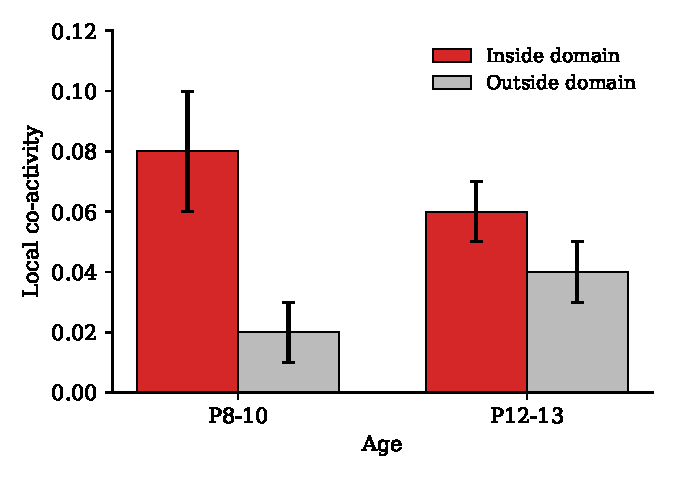
\includegraphics[width=0.55\textwidth]{figures/fig_coactivity.pdf}
\caption{Local co-activity was consistently higher inside than outside dendritic domains at both ages (P8--10: in-domain $0.08 \pm 0.02$, out-of-domain $0.02 \pm 0.01$; P12--13: in-domain $0.06 \pm 0.01$, out-of-domain $0.04 \pm 0.01$; mean $\pm$ SEM; $n = 213$ in-domain, $173$ out-of-domain synapses; Mann--Whitney $U$ test).}
\label{fig:coactivity}
\end{figure}

\begin{table}[htbp]
\centering
\caption{Local co-activity inside versus outside dendritic domains, by age. Values are mean $\pm$ SEM. Sample sizes are pooled across all ages ($n = 213$ in-domain and $n = 173$ out-of-domain synapses, Mann--Whitney $U$ test).}
\label{tab:coactivity}
\begin{tabular}{lcc}
\toprule
Age & In-domain co-activity & Out-of-domain co-activity \\
\midrule
P8--10 & $0.08 \pm 0.02$ & $0.02 \pm 0.01$ \\
P12--13 & $0.06 \pm 0.01$ & $0.04 \pm 0.01$ \\
\bottomrule
\end{tabular}
\end{table}

\subsection{Local co-activity correlates with synapse stabilization}

Finally, we asked how homogeneous starting material could become partitioned into functionally distinct domains. Guided by prior evidence that local co-activity drives the clustering of developing synapses \citep{winnubst2012synaptic}, we examined whether co-activity with neighbors predicted how individual synapses changed their transmission over time. For each synapse, we computed the Mann--Kendall statistic of its transmission frequency across the recordings of an experiment: positive scores indicate monotonic increases, negative scores indicate decreases, and zero indicates stability.

On average, synapses located inside domains had higher Mann--Kendall scores than those located outside, with out-of-domain synapses tending toward decreasing activity ($n = 213$ in-domain and $n = 173$ out-of-domain synapses; independent Student's $t$-test). Going further, the Mann--Kendall score of each synapse correlated positively with its local co-activity with neighbors within 10 $\mu$m proximally and distally (linear regression restricted to synapses with transmission frequency of at least 0.6 min$^{-1}$). In other words, synapses that were synchronized with their neighbors tended to strengthen or at least remain stable, while synapses that were out of sync with their neighbors tended to weaken. This pattern provides a direct developmental correlate of the Hebbian-like rule that has been proposed to organize clustered inputs in the cortex, and it explains how scattered synapses become sorted into co-active domains during the second postnatal week (Figure~\ref{fig:model}).

\begin{figure}[htbp]
\centering
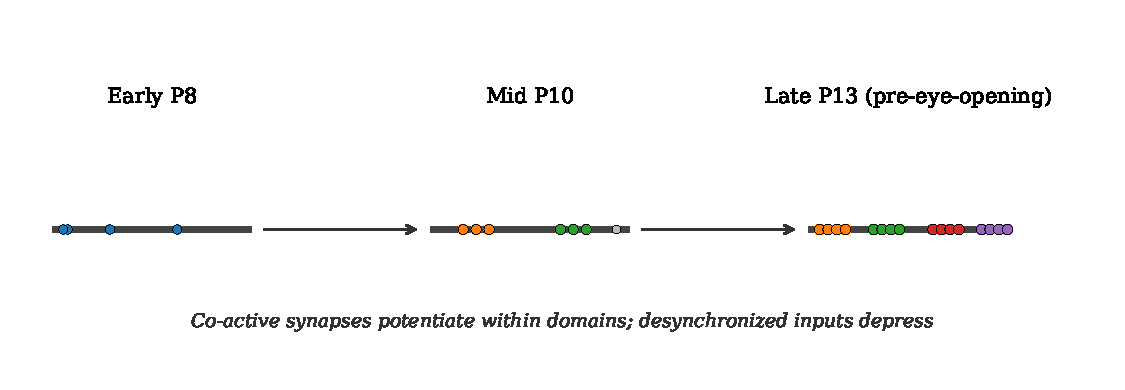
\includegraphics[width=0.95\textwidth]{figures/fig_domain_schematic.pdf}
\caption{Model of dendritic-domain assembly before eye opening. At P8, only a few active synapses are scattered across the developing dendrite. During the second postnatal week, synapses sort into functionally distinct domains: in-sync synapses stabilize or potentiate while desynchronized inputs undergo depression. By P12--13, dendrites are largely covered by domains of neighbors whose co-activity within a domain exceeds co-activity across domains.}
\label{fig:model}
\end{figure}

Collectively, these results show that visual cortical neurons establish functional synaptic inputs at a high rate during the week before eye opening, and that those inputs become organized into spatially and functionally distinct dendritic domains. Synchronization with neighbors is associated with synapse stabilization, suggesting that the same local-correlation rule that is thought to govern clustering in the mature cortex is already in play during this developmental window. The Discussion that follows places these findings in the context of adult clustering, candidate plasticity mechanisms, and the sensory computations that these pre-existing domains may be poised to support.

\section{Discussion}

We used simultaneous whole-cell voltage-clamp and two-photon dendritic imaging in vivo to map functional synaptic inputs across layer 2/3 pyramidal cell dendrites of the mouse primary visual cortex during the week leading up to eye opening. Our central finding is that clustered synaptic inputs assemble into spatially and functionally distinct dendritic domains before the first visual experience. Synapse density and per-synapse transmission frequency rose steeply across the second postnatal week, spine and shaft synapses showed stable rate asymmetries (spine $0.55 \pm 0.09$ vs.\ shaft $0.16 \pm 0.03$ min$^{-1}$ at P8--10; spine $0.67 \pm 0.07$ vs.\ shaft $0.23 \pm 0.03$ min$^{-1}$ at P12--13), and the fraction of dendritic length covered by domains more than doubled ($27.2\%$ to $61.3\%$). Within each domain, local co-activity was higher than between domains, and synapses synchronized with their neighbors tended to stabilize or strengthen, as summarized by their Mann--Kendall plasticity scores. These observations provide a developmental account of how the clustered input architecture of adult cortex \citep{iacaruso2017synaptic,wilson2016orientation,takahashi2012locally} is built.

A conspicuous feature of our data is the long-tailed distribution of per-synapse transmission rates: most synapses are quiet while a minority dominate the input stream. Because the presynaptic population -- other layer 2/3 pyramidal neurons -- fires homogeneously during neonatal spontaneous network events \citep{siegel2012peripheral,ackman2012retinal}, this heterogeneity cannot be inherited from firing-rate differences among presynaptic partners. The simpler explanation is that individual synapses differ in their presynaptic release probabilities, in line with paired-recording measurements showing that release-probability variability dominates synaptic strength differences between cortical neurons \citep{markram1997physiology,silver2003high}. Our previous work on developing visual cortex further showed that per-synapse transmission frequency is highly plastic and regulated by local synaptic interactions \citep{winnubst2012synaptic}. Together this evidence argues that release-probability heterogeneity provides the dynamic range the developing circuit needs to tune individual connection strengths in response to fine-grained local activity, and that this heterogeneity is actively shaped by the local-co-activity rule we document here.

A second noteworthy quantitative observation is that the mean number of synapses per domain grew from roughly three to six during the second postnatal week. In mature cortex, functionally connected pyramidal neurons typically share fewer than ten synapses, and those synapses are generally spread across different dendrites \citep{markram1997physiology,silver2003high}. However, multi-contact innervation of a single dendritic segment by a single axon is not unusual in the mature circuit and is plausibly more common during development when synapse density is rising sharply. Our dataset probably contains such redundant synapses. The activity-based plasticity rule we describe -- synchronous neighbors potentiate or stabilize while asynchronous neighbors depress -- supplies a natural mechanism for assembling multi-contact inputs from presynaptic partners whose activity correlates with the local network, consistent with proposals linking partner selection to coincident activity.

What features of the sensory world could these pre-experience domains already encode? In mature V1, neighboring synapses are more likely to share receptive-field structure -- either retinotopic location and receptive-field similarity in mouse \citep{iacaruso2017synaptic} or orientation preference in ferret \citep{wilson2016orientation}. Before eye opening, patterned spontaneous activity travels along the visual pathway: retinal waves transmit retinotopic, direction, and orientation information to the cortex \citep{ackman2012retinal}, and local cortical network events shape neonatal V1 dynamics in ways that survive the removal of retinal drive \citep{siegel2012peripheral}. The plasticity rule our measurements implicate -- local co-activity biases synapse stabilization -- can readily translate these activity statistics into dendritic architecture. Domains are thus well-positioned to encode a first approximation of the neighborhood relationships of presynaptic neurons in visual space, providing ready-made subunits for the supralinear integration that dendritic spikes and spine amplification support in the adult cortex \citep{losonczy2006integrative,harnett2012synaptic,smith2013dendritic,lavzin2012nonlinear,poirazi2003pyramidal,larkum2013cellular}. Our observation that functional synapses form in defined domains while other stretches remain synapse-free at the start of the second postnatal week further indicates that clustering is an active organizational principle rather than a by-product of smooth gradients in synapse density.

Several limitations of this study should be kept in view. Our recordings were carried out under light isoflurane anesthesia. We previously showed that this level of anesthesia reduces the frequency of spontaneous network events but does not alter their participation rates or event amplitudes, and that synaptic input organization is similar in vivo under light anesthesia and in slice cultures \citep{siegel2012peripheral}. We cannot therefore entirely rule out subtle effects of anesthesia on the exact dynamics we observe, but the core architectural features of clustering and domain formation are unlikely to be artifacts of the recording state. A second limitation is the modest number of animals ($n = 11$) and the confinement to apical dendrites of layer 2/3 pyramidal cells. Broader sampling across cortical layers, basal dendrites, and brain regions would test whether domain assembly is a general cortical developmental motif. Finally, because the axial resolution of two-photon microscopy is worse than its lateral resolution, a small number of spines hidden in the z-dimension may have been misclassified as shaft synapses; this would, if anything, underestimate the contrast between spine and shaft rates.

Looking forward, our findings raise three lines of inquiry. First, the molecular mechanisms that translate local co-activity into synapse stabilization in this developmental window remain to be tied directly to domain assembly; the BDNF/proBDNF-based push--pull plasticity that has been implicated in synaptic clustering in younger tissue \citep{winnubst2012synaptic} is a natural candidate. Second, it will be important to test whether the functional domains we describe pre-exist the receptive-field organization that emerges after eye opening, or whether eye opening reconfigures them on a short timescale. Third, the interplay between excitatory domains and the rapid remodeling of inhibitory synapses documented in mature cortex \citep{villa2016inhibitory} could further sculpt the subcellular geometry of inputs once vision begins. Regardless of how these questions resolve, the central point is that functional synaptic clustering in visual cortex is already in place before the eyes open. Spontaneous activity, operating on an activity-dependent plasticity rule local to each dendritic segment, is sufficient to construct the computational subunits on which cortical visual processing will then depend.

\bibliographystyle{unsrtnat}
\bibliography{references}

\end{document}
